\documentclass[a4paper]{article}
\usepackage{latexsym}
\usepackage[a4paper]{geometry}
\usepackage{color}
\usepackage{listings}
\usepackage[pdftex]{graphicx}
\usepackage{float}

\definecolor{Blue}{rgb}{0,0,0.5}
\definecolor{Green}{rgb}{0,0.75,0.0}
\definecolor{LightGray}{rgb}{0.6,0.6,0.6}
\definecolor{DarkGray}{rgb}{0.3,0.3,0.3}
\lstset{language=Matlab,
   keywords={function,uint8,uint16,uint32,double,break,case,catch,continue,else,elseif,end,for,global,if,otherwise,persistent,return,switch,try,while},
   basicstyle=\ttfamily\small,
   breaklines=true,
   keywordstyle=\bfseries\color{Blue},
   commentstyle=\itshape\color{LightGray},
   stringstyle=\color{Green},
   numbers=left,
   numberstyle=\tiny\color{DarkGray},
   stepnumber=1,
   numbersep=10pt,
   backgroundcolor=\color{white},
   tabsize=2,
   showspaces=false,
   showstringspaces=false,
   captionpos=b}

%Boldface text for type writer font
\usepackage{bold-extra} %\DeclareFontShape{OT1}{cmtt}{bx}{n}{<5><6><7><8><9><10><10.95><12><14.4><17.28><20.74><24.88>cmttb10}{}

%Break words properly at the end of a line (which isn't sloppy...)
\sloppy

%Use command \exercise for each exercise
\newcounter{exerciseCount}
\setcounter{exerciseCount}{0}
\newcommand{\exercise}[1]{\addtocounter{exerciseCount}{1} \noindent \medskip {\large \textsf{\textbf{Exercise \arabic{exerciseCount} \--- #1}}} \par}
\renewcommand{\theenumi}{\textsf{\textbf{\alph{enumi}}}}

%Use command \code for code snippets
\newcommand{\code}[1]{\textnormal{\texttt{#1}}}

\title{\textsf{Image Processing \\ lab 5}}
\author{Klaas Kliffen \and Jan Kramer}
\date{\today}

\begin{document}
\maketitle

\exercise{Edge detection}
\begin{enumerate}
\item
%\lstinputlisting{../lab5ex1/IPMarrHilderth.m}
\item
\begin{figure}[H]
\centering
\begin{tabular}{cc}
    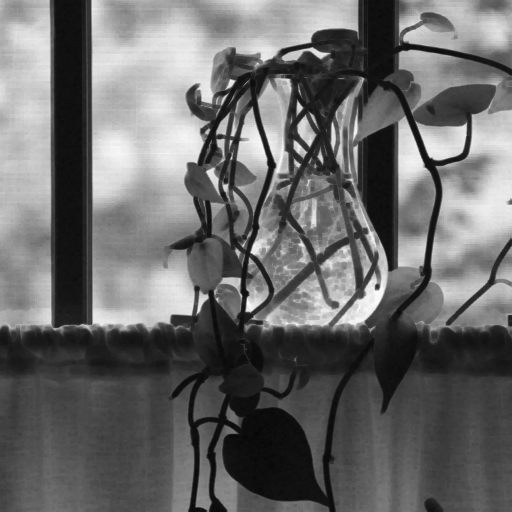
\includegraphics[width=0.3\textwidth]{../lab4ex2/gerode.png} & 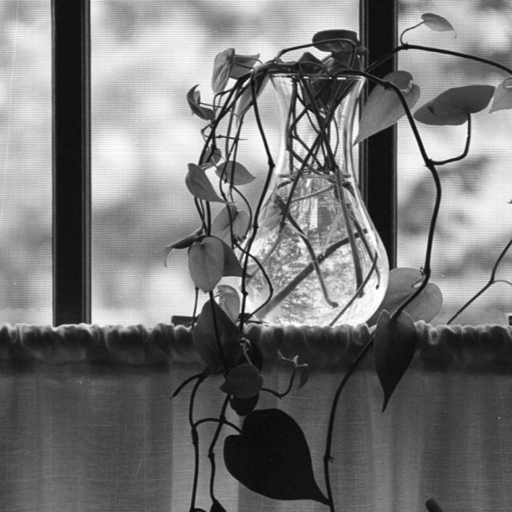
\includegraphics[width=0.3\textwidth]{../lab4ex2/vase.png} \\
    The erosion & Original image \\
\end{tabular}
\caption{TODO}
\label{fig:marrhil}
\end{figure}
\end{enumerate}


\exercise{Region splitting and merging}
\begin{enumerate}
\item There are two main objects in the scene, the tiger and the sky. The tiger consists of a large range of grey levels and complex patterns.
The sky however is smooth and consists of a well defined range of grey levels. Therefor it less complex to define a piece of sky.
Opening Figure \ref{fig:tiger} in an image editor gave the value 107 as a lower bound for the dark regions and 168 for brighter regions.
Therefor a suitable predicate would be that all pixels in the regions are with these bounds. For the actual implementation a slightly larger bound is used,
since some areas where still a bit brighter than measured and therefor the final bounds used are $[100, 180]$.
\begin{figure}[H]
\centering
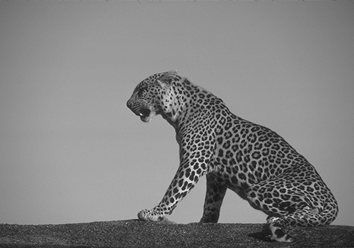
\includegraphics[width=0.4\textwidth]{../lab5ex2/tiger.png} \\
\caption{The original image with the tiger}
\label{fig:tiger}
\end{figure}

\item The predicate implementation is quite simple. It mainly consists of two large matrices used to detect values above the lower bound an below the higher bound.
The difference is taken and should sum to 0 if all values in the region are with the bounds. However, since the image is padded by the split and merge algorithm to a power of two.
It is possible that around the border of an image some values are zero in a region.
This is avoided by setting all pixels in the region with a zero grey level to 128 (a value in between the bounds).

\lstinputlisting{../lab5ex2/IPpredicate.m}



\begin{figure}[H]
\centering
\begin{tabular}{ccc}
    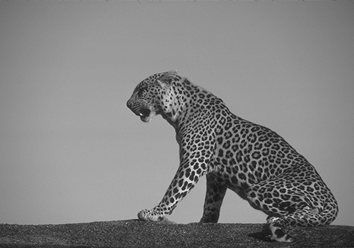
\includegraphics[width=0.3\textwidth]{../lab5ex2/tiger.png} & 
\includegraphics[width=0.3\textwidth]{../lab5ex2/block-1.png} & 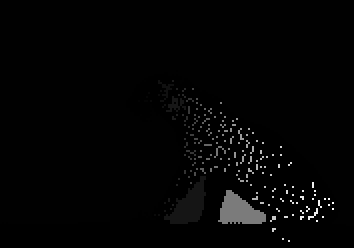
\includegraphics[width=0.3\textwidth]{../lab5ex2/block-2.png} \\
    Original image & Block size 1& Block size 2 \\
        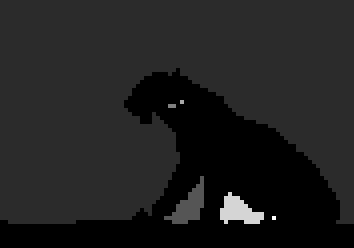
\includegraphics[width=0.3\textwidth]{../lab5ex2/block-4.png} & 
\includegraphics[width=0.3\textwidth]{../lab5ex2/block-8.png} & 
\includegraphics[width=0.3\textwidth]{../lab5ex2/block-16.png} \\
    Block size 4 & Block size 8& Block size 16 \\
\end{tabular}
\caption{The partitioning scheme on the tiger image with different minimum block sizes}
\label{fig:blocks}
\end{figure}

In Figure \ref{fig:blocks} the results can be seen with various minimum block sizes. The best block size for this particular image seems to be a size of 4.
Anything smaller has too much connected blocks, where the tiger is completely invisible. 
When comparing the block size of 8 with 4, the tiger has no gaps, but the contour is less detailed. A block size of 4 still can be recognized as a tiger.
A block size of 16 is useless, since it there is no more detail to be found in the image.

\end{enumerate}

\exercise{Fourier descriptors}
\begin{enumerate}
\item
The starting point of the boundary is determined by systematically scanning each horizontal row.
It starts in the center and checks if the row has values other than the background value.
If not, two new rows are checked, each at a quarter of the image, until there are no more rows to scan and it will throw an error.
Having found the starting point, the \lstinline|bwtraceboundary|  function is called.
\lstinputlisting{../lab5ex3/IPcontour.m}
\item The starting point of the boundary using the method described above is at x: 25, y: 111.
The complete boundary can be seen in Figure \ref{fig:lincoln}
\begin{figure}[H]
\centering
\begin{tabular}{cc}
    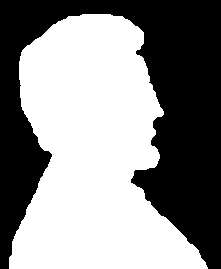
\includegraphics[width=0.3\textwidth]{../lab5ex3/lincoln.png} & 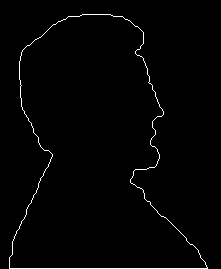
\includegraphics[width=0.3\textwidth]{../lab5ex3/contour-410.png} \\
    The original image & The contour \\
\end{tabular}
\caption{The contour of the silhouette of Lincoln}
\label{fig:lincoln}
\end{figure}

\item
The Fourier descriptors are calculated by the build in function fft.
Since the center of the array resemble the higher frequencies, the number of descriptors to be kept is at the start and the end of the array.
With a simple for loop, each of the center values can be set to 0.
The resulting approximating boundary is then retrieved by the rounding the real part of the inverse Fourier transformation.

\lstinputlisting{../lab5ex3/IPfourierdescr.m}
\item

\begin{figure}[H]
\centering
\begin{tabular}{ccc}
    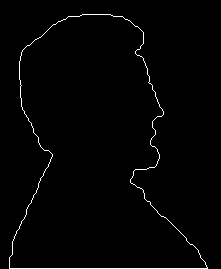
\includegraphics[width=0.3\textwidth]{../lab5ex3/contour-410.png} & 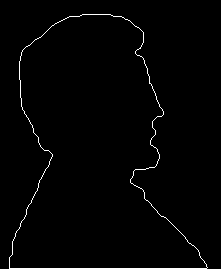
\includegraphics[width=0.3\textwidth]{../lab5ex3/contour-100.png} & 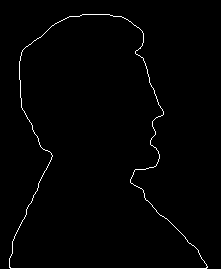
\includegraphics[width=0.3\textwidth]{../lab5ex3/contour-75.png} \\
    Original contour (410 descriptors) & 100 descriptors & 75 descriptors \\
        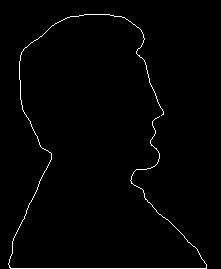
\includegraphics[width=0.3\textwidth]{../lab5ex3/contour-50.png} & 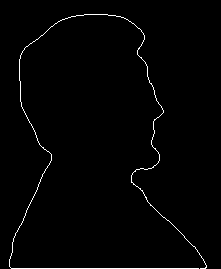
\includegraphics[width=0.3\textwidth]{../lab5ex3/contour-38.png} & 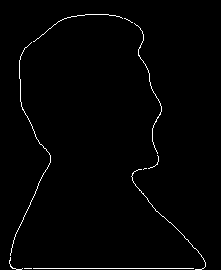
\includegraphics[width=0.3\textwidth]{../lab5ex3/contour-25.png} \\
    50 descriptors &  38 descriptors & 25 descriptors \\
\end{tabular}
\caption{The contour of the Lincoln silhouette using different amounts of Fourier descriptors}
\label{fig:contour}
\end{figure}

As can be seen in Figure \ref{fig:contour}, the minimal number of descriptors needed for a recognizable silhouette is somewhere around 38. 
Using less descriptors will smooth the surface, where at 25 descriptors most features are smoothed and it effort to recognize the silhouette of Lincoln.

\end{enumerate}

\section*{Task distribution}

\begin{table}[H]
\centering
\begin{tabular}{ccccc}
ex1 & design & implementation & answers questions & writing report \\
\hline
Klaas & 20\% & 10\% & 20\% & 30\% \\
\hline
Jan & 80\% & 90\% & 80\% & 70\% \\
\end{tabular}
\end{table}

\begin{table}[H]
\centering
\begin{tabular}{ccccc}
ex2 & design & implementation & answers questions & writing report \\
\hline
Klaas & 50\% & 80\% & 75\% & 75\% \\
\hline
Jan & 50\% & 20\% & 25\% & 25\% \\
\end{tabular}
\end{table}

\begin{table}[H]
\centering
\begin{tabular}{ccccc}
ex3 & design & implementation & answers questions & writing report \\
\hline
Klaas & 80\% & 75\% & 75\% & 80\% \\
\hline
Jan & 20\% & 25\% & 25\% & 20\% \\
\end{tabular}
\end{table}

\end{document}
